\chapter{作品概述}\label{ux7b2cux4e00ux7ae0-ux4f5cux54c1ux6982ux8ff0}

本章主要介绍 V-Guard
作品提出的背景、已有研究基础、作品特色和应用前景。首先分析生成式语音技术发展带来的声音资产安全风险，然后概括语音合成与语音隐私保护领域的相关工作，最后说明本作品在发布前主动防护、联合保护机制、听感可用性和系统闭环方面的主要特点。

\section{作品背景与意义}\label{ux4f5cux54c1ux80ccux666fux4e0eux610fux4e49}

近年来，深度学习、自监督语音表征学习和生成式人工智能技术持续推动语音合成能力发展。早期语音合成系统通常依赖人工设计的声学特征、统计模型或较复杂的文本前端规则，而现代神经网络语音合成系统已经能够生成自然度较高、情感表达较丰富、说话人相似度较强的语音内容。随着模型结构和训练数据规模不断扩大，语音合成系统不再只用于无身份特征的普通播报，也逐渐具备根据少量参考语音复刻目标说话人声音特征的能力{[}1-8{]}。

从实际风险看，语音克隆技术降低了声音仿冒的门槛。攻击者不一定需要长期接触目标用户，也不一定需要获取高质量录音棚语音。公开短视频、直播录屏、采访片段、播客节目、在线课程、会议录音、客服电话和企业宣传视频中都可能包含目标说话人的真实语音片段。这些语音一旦被批量收集，就可能被用于构造语音克隆参考样本，进一步生成与目标说话人高度相似的合成语音。对于个人用户而言，这可能造成熟人诈骗、虚假言论伪造和身份冒用；对于企业而言，这可能导致客服声音仿冒、品牌语音资产滥用和定向社会工程攻击；对于内容平台而言，这也会增加虚假音频传播、内容审核和生成式人工智能治理的压力。

例如，声音资产的商业价值正面临大规模非法滥用：2023 年，AI
生成的伪造歌曲``Heart on My Sleeve''因逼真模仿了 Drake 和 The Weeknd
的嗓音而火爆全网，引发了关于公众人物声音资产所有权与数字版权的激烈法律争议;在企业级应用中，`CEO
欺诈'已成为重大安全威胁：2019 年，一家英国能源公司遭 AI
语音伪造欺诈，损失22万欧元。攻击者利用语音合成技术模仿母公司 CEO
的音色与韵律，向财务部门下达紧急转账指令。


\begin{figure}[htbp]
  \centering
  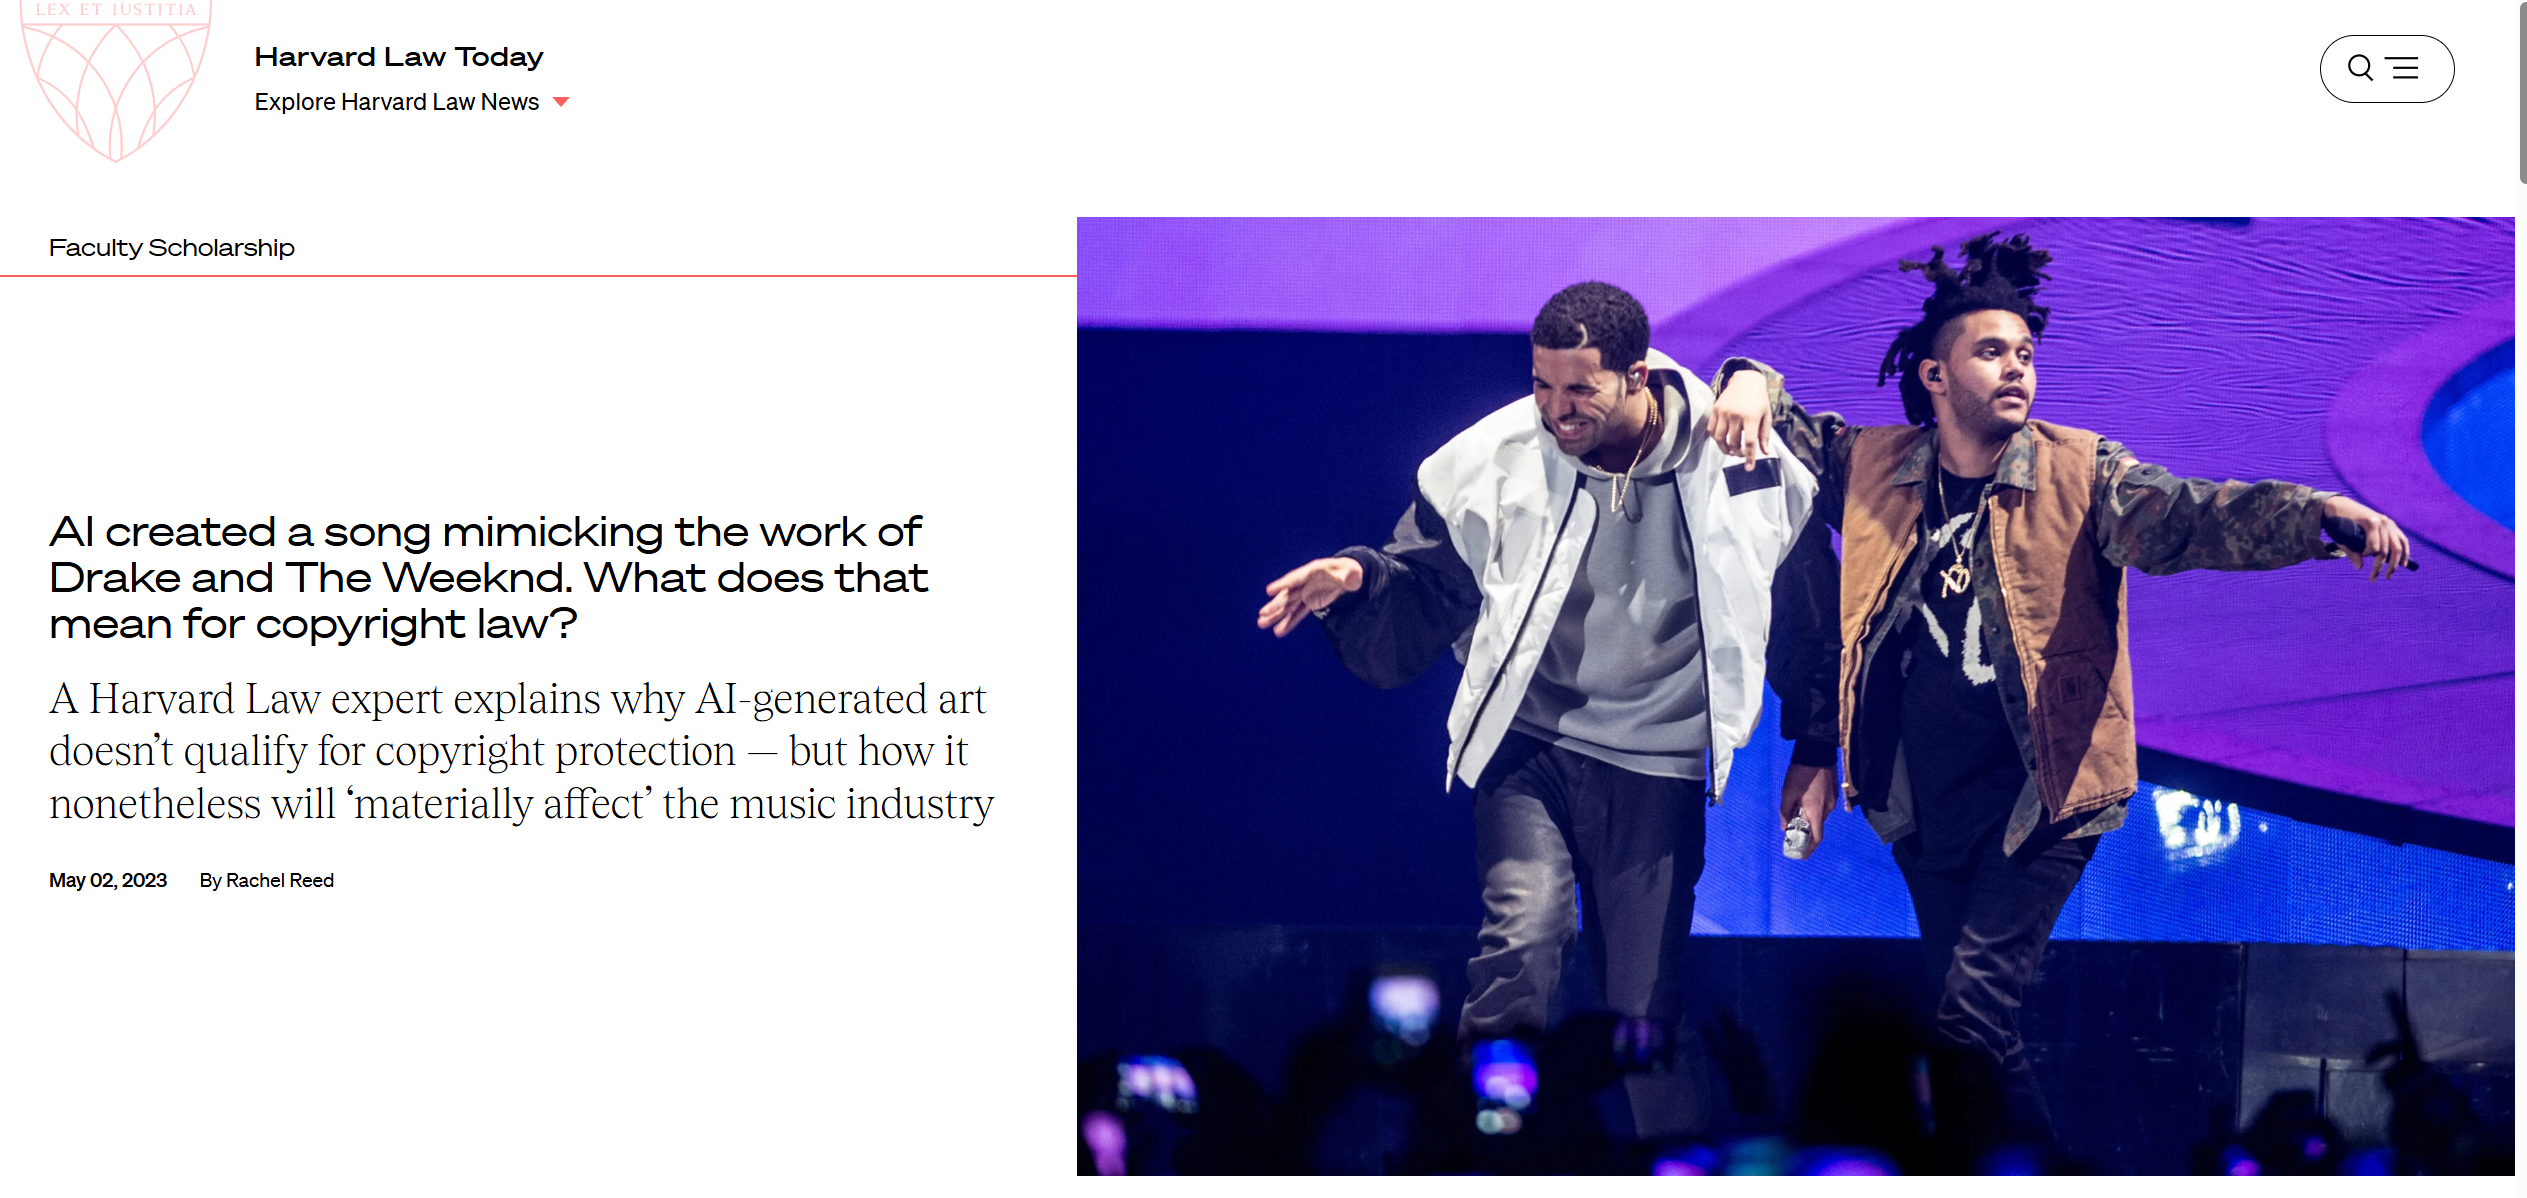
\includegraphics[width=\textwidth,height=0.72\textheight,keepaspectratio]{figures/image1.png}
  \caption{Drake 与 The Weeknd 的 AI 伪造歌曲事件\textsuperscript{{[}9{]}}}
  \label{fig:1-1}
\end{figure}


\begin{figure}[htbp]
  \centering
  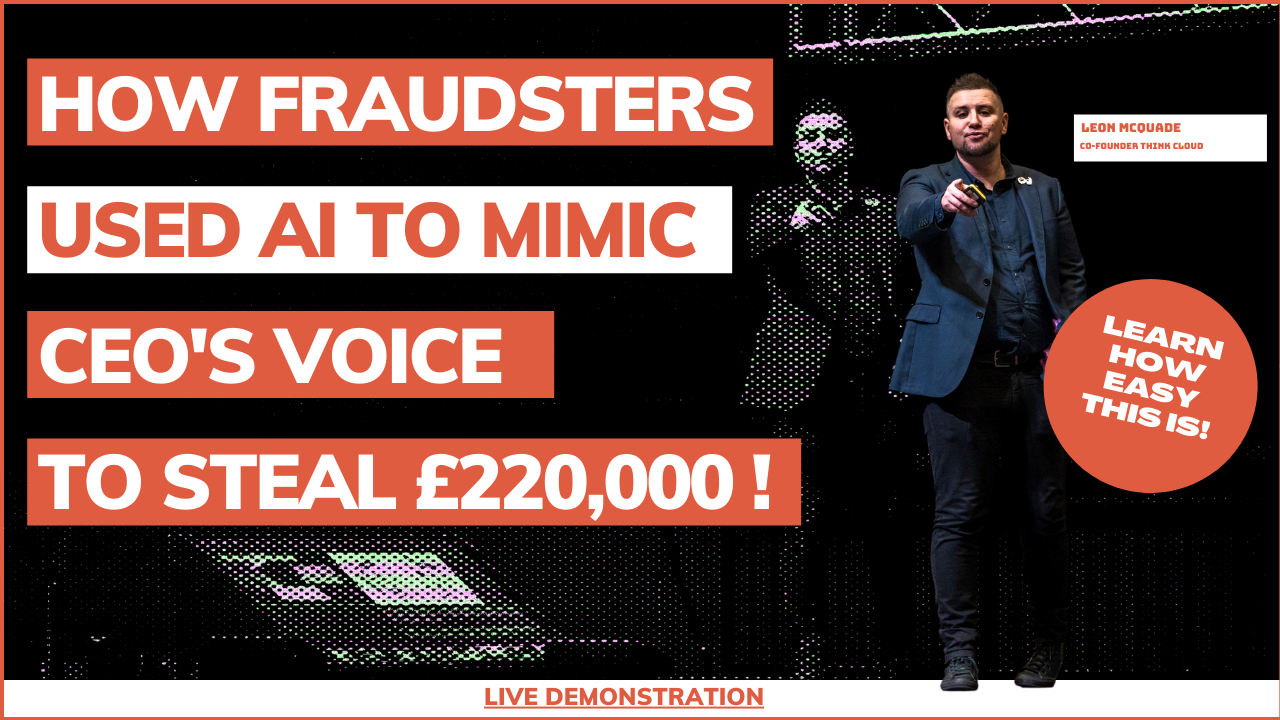
\includegraphics[width=\textwidth,height=0.72\textheight,keepaspectratio]{figures/image2.png}
  \caption{英国能源公司``CEO 欺诈''案\textsuperscript{{[}10{]}}}
  \label{fig:1-2}
\end{figure}

此类事件直观展现了生成式 AI
可以利用现有语音样本在短时间内精准模拟韵律与语调，绕过传统的内部身份审核机制，侵占个人声音权，从而论证了
V-Guard 这种能够从源头削弱声音被复刻利用的技术方案具有显著的落地价值。

当前语音克隆风险主要可以概括为三类。

第一类是零样本语音克隆，即攻击者只需要提供短时间参考音频和目标文本，就可能合成具有相似声音特征的语音。VALL-E
等神经音频编码语言模型表明，离散音频编码可以被用于条件语言建模式的零样本语音合成，并能够根据短参考语音生成个性化语音\textsuperscript{{[}5{]}}。

第二类是少样本或微调式语音克隆，即攻击者收集多条目标说话人语音后，对模型进行适配、微调或条件建模，从而更稳定地学习目标说话人的声音身份信息{[}8,11{]}。

第三类是基于大语言模型的语音合成，即系统将连续语音转换为离散语音
token，再由语言模型或生成模型完成后续建模与合成。CosyVoice
等系统进一步说明，监督语义 token
与大语言模型结合后，可以提升零样本语音合成中的内容一致性和说话人相似度\textsuperscript{{[}6{]}}。

上述风险说明，语音克隆系统并不是只依赖某一个单一特征。概括来说，机器至少需要从参考音频中提取两类信息：一类是``说了什么''，包括语音内容、发音单元、文本转写、语义
token
和文本---发音对齐关系；另一类是``是谁在说、怎么说''，包括说话人身份、音色、韵律、风格、情绪和声学环境等声音条件。前者构成语义表示链路，后者构成声音身份特征链路。如果防护方法只影响自动语音识别结果，而不影响声音身份表示，攻击者仍可能从参考音频中提取目标说话人的声音条件；如果防护方法只降低声纹相似度，而不影响语义内容和文本对齐关系，攻击者仍可能在自动标注或微调场景中构造可用训练样本。因此，真实语音克隆风险要求防护系统同时关注这两类机器依赖。

现有治理手段多集中于事后环节。例如，深度伪造检测模型可以在音频生成后判断其是否存在伪造痕迹，水印和溯源技术可以辅助平台识别生成内容来源，内容审核机制可以在平台传播阶段拦截高风险音频。这些方法对平台治理和事后追责具有价值，但它们通常无法阻止攻击者在前端收集真实语音样本。一旦原始声音资产被公开暴露，攻击者就可能在检测系统介入之前完成采集、编码和建模。因此，仅依赖事后检测并不能充分解决声音资产源头泄露问题。

基于上述背景，本作品采用发布前主动防护思路。主动防护的目标不是在伪造语音生成后再判断真假，而是在用户公开发布或外发真实语音之前，为原始音频生成受保护音频。该音频对人耳应尽量保持自然、可懂和可用，但在机器模型看来，其语义表示、声音身份表示或离散语音
token
可能发生偏移，从而削弱未授权语音克隆系统对原始声音资产的稳定提取能力。由此，V-Guard
试图在声音数据源头增加一道主动保护层，为个人声音隐私、企业声音资产管理和生成式语音安全治理提供可落地的系统方案。


\begin{figure}[htbp]
  \centering
  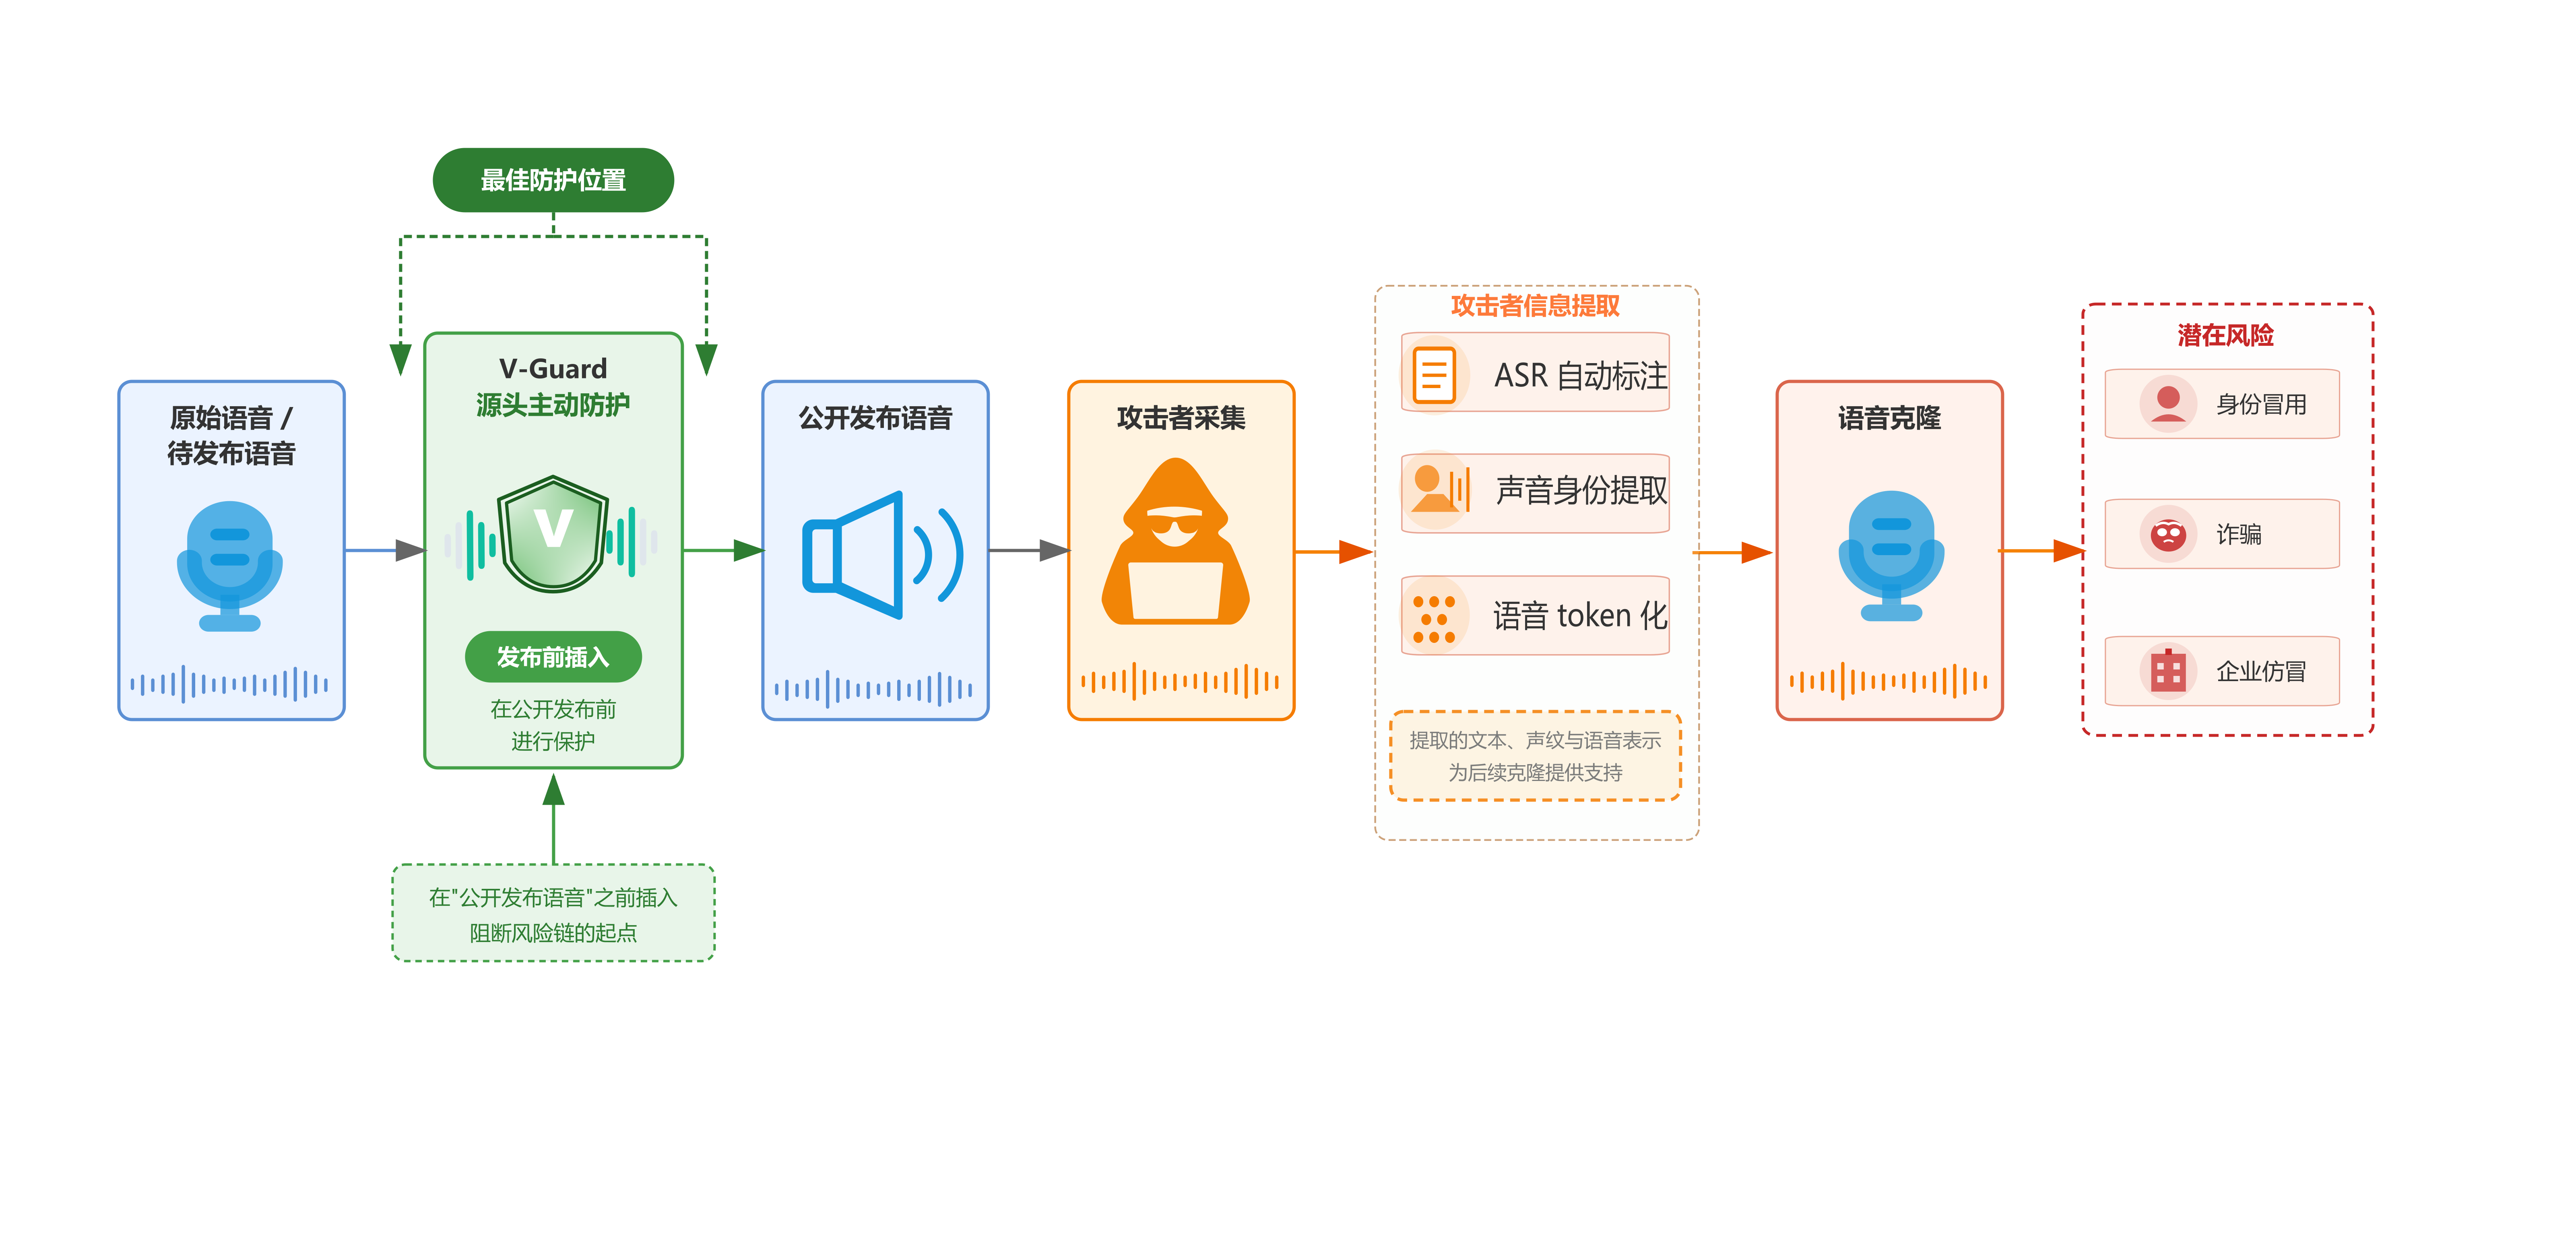
\includegraphics[width=\textwidth,height=0.72\textheight,keepaspectratio]{figures/image3.png}
  \caption{语音克隆风险链路与 V-Guard 源头防护位置示意图}
  \label{fig:1-3}
\end{figure}

\section{相关工作}\label{ux76f8ux5173ux5de5ux4f5c}

语音安全问题与语音合成技术发展密切相关。本节从语音合成和语音隐私保护两个方面概括已有工作，为后续章节介绍相关技术和系统实现提供基础。

\subsection{语音合成}\label{ux8bedux97f3ux5408ux6210}

语音合成技术的目标是将文本或其他输入条件转换为自然语音。传统语音合成方法包括拼接式语音合成、参数式语音合成和统计参数语音合成。这类方法通常依赖人工设计的语言学特征、声学特征和声码器结构，能够完成基本播报任务，但在自然度、情感表达、韵律变化和说话人个性化方面存在限制。

随着深度学习发展，神经网络语音合成逐渐成为主流方向。典型系统通常先将文本转换为声学表示，再由声码器生成波形。Tacotron
2
采用从字符序列到梅尔频谱，再由神经声码器生成波形的结构，推动了端到端神经语音合成的发展\textsuperscript{{[}1{]}}。FastSpeech
和 FastSpeech 2
等非自回归语音合成方法进一步提升了生成速度和稳定性\textsuperscript{{[}2-3{]}}。VITS
则通过变分推断、标准化流和对抗训练实现端到端文本到语音合成，使语音合成系统在自然度和工程简化方面继续发展\textsuperscript{{[}4{]}}。

在此基础上，语音合成逐渐从``生成自然语音''扩展到``生成具有特定说话人特征的语音''。零样本语音克隆和少样本语音克隆的出现，使模型可以根据短参考音频提取目标说话人的声音条件，并结合输入文本生成相似语音。VALL-E
将文本到语音合成建模为基于神经音频编码离散码的条件语言建模任务，展示了语音
token
与语言模型结合后的零样本合成能力\textsuperscript{{[}5{]}}。CosyVoice
则通过监督语义 token 和大语言模型式文本到 token
生成，提高了零样本语音合成中的内容一致性和说话人相似度\textsuperscript{{[}6{]}}。这些工作一方面推动了语音生成技术进步，另一方面也说明真实语音样本可能成为未授权语音克隆的重要入口{[}7-18{]}。

因此，在语音合成技术持续发展的背景下，声音资产安全需要从传统内容审核和事后检测进一步前移到语音发布前防护。只有在声音样本被采集、编码和建模之前加入保护机制，才能更直接地降低未授权语音克隆的源头风险。

\subsection{语音隐私保护}\label{ux8bedux97f3ux9690ux79c1ux4fddux62a4}

现有语音隐私保护和语音伪造治理方法大体可以分为三类：被动检测、水印溯源和主动防护。

被动检测方法主要在合成语音已经产生之后，通过深度伪造检测模型判断音频是否由生成模型合成。这类方法适合平台审核、内容治理和事后追责，但检测效果往往受训练数据、生成模型更新、压缩转码和真实环境噪声影响。当生成模型持续迭代时，检测模型也需要不断更新，否则可能出现漏检或误检。

水印溯源方法通常在生成音频时嵌入可识别标记，或在平台侧记录生成内容来源。这类方法有助于追踪合成语音来源，但前提是生成系统或平台本身配合嵌入水印。对于攻击者私下使用开源模型、本地模型或未经监管的商业接口生成伪造语音的情况，水印溯源难以覆盖全部风险。

主动防护方法则将作用位置前移到真实语音发布之前。其基本思路是在原始音频中加入人耳不易察觉或可接受的保护扰动，使其仍可用于正常收听和传播，但降低机器模型对关键语音信息的稳定提取能力。AntiFake
提出利用对抗音频预防未授权语音合成，使攻击者基于受保护语音生成的伪造音频不再像受害者本人\textsuperscript{{[}19{]}}。E2E-VGuard
进一步面向生产级大语言模型语音合成和自动语音识别驱动的端到端场景，讨论了主动防护在真实语音克隆流程中的作用位置\textsuperscript{{[}23{]}}。这些工作说明，主动防护能够与被动检测、水印溯源形成互补，为声音资产提供更靠前的保护层。相关语音隐私和主动防护研究还包括语音转换防护、不可学习语音样本、语音匿名化和商用
ASR 隐私保护等方向{[}20-22,24-27{]}。

本作品属于主动防护范畴，但并不将目标限定为某一个单一语音合成模型。V-Guard
面向真实使用场景中的不确定攻击流程，将语义表示链路、声音身份特征链路和听感约束共同纳入系统设计。系统既关注机器是否还能稳定理解``说了什么''，也关注机器是否还能稳定提取``是谁在说、怎么说''，同时通过网页端功能闭环使防护过程具备可操作性和可展示性。

\section{作品特色描述}\label{ux4f5cux54c1ux7279ux8272ux63cfux8ff0}

本作品设计并实现了一套面向声音资产发布前防护的主动式语音防克隆系统V-Guard，系统围绕语音克隆对参考音频的两类关键机器依赖，通过语义表示链路和声音身份表示链路联合施加保护扰动，同时引入心理声学约束控制扰动对正常听感的影响，并将上述机制封装为包含接入、保护、评估和导出的完整网页端平台。以下从四个方面介绍本作品的主要特色。

\subsection{源头主动防护}\label{ux6e90ux5934ux4e3bux52a8ux9632ux62a4}

V-Guard
将防护位置前移到语音公开发布或外发之前。用户在上传短视频、播客、有声读物、企业宣传音频、客服语音或会议录音之前，可以先通过系统生成受保护音频，再将其用于后续使用。与事后检测不同，主动防护并不等待伪造语音出现后再进行识别，而是尽量在原始声音样本被机器采集和建模之前降低其可利用性。

这一前置性设计不依赖对特定克隆模型的先验知识，能够同时覆盖零样本、少样本和微调式等多种克隆攻击方式。同时，这一设计更符合声音资产的特殊属性，声音不同于密码、验证码或密钥，它在内容创作、在线交流和公共传播中经常需要被公开使用，而且一旦公开传播就很难完全撤回，且完全隐藏声音并不现实。

\subsection{基于语义与声音身份表示的联合保护}\label{ux57faux4e8eux8bedux4e49ux4e0eux58f0ux97f3ux8eabux4efdux8868ux793aux7684ux8054ux5408ux4fddux62a4}

语音克隆系统通常同时依赖语义信息和声音身份信息。语义信息决定机器如何理解语音内容、发音结构和文本对齐关系；声音身份信息决定机器如何提取说话人身份、音色、韵律、风格和声学条件。仅影响其中一个方面，往往不足以覆盖真实语音克隆流程。

本作品同时考虑上述两类链路。在语义链路上，防护目标从传统的ASR文本输出层面下沉至语音编码器的中间表示层面。系统以S3
Tokenizer、HuBERT、Whisper等模型作为语义代理模型，通过扰动连续语义表示影响离散语音token的量化结果，从更底层的表示空间破坏语音内容的可理解性。在声音身份链路上，通过集成VITS、GPT-SoVITS、CosyVoice
CAM++、StyleTTS2风格编码器、WavLM和MFCC等多种编码器作为代理模型，使保护扰动在多个身份表示空间中同时偏离原始说话人，并支持无目标与有目标两种保护模式。这种多编码器集成的方式能够覆盖不同模型对声音身份的提取方式，降低对单一模型的依赖，从而提升对未知语音克隆系统的防护迁移性。两类链路共享同一个保护扰动，在优化过程中共同驱动扰动生成，使受保护音频同时在语义可理解性和身份可识别性两个维度上偏离原始音频。

\subsection{心理声学约束}\label{ux5fc3ux7406ux58f0ux5b66ux7ea6ux675f}

主动防护不能简单等同于向音频中加入强噪声。如果保护后的音频出现明显底噪、失真、语义不可辨识或播放体验下降，即使机器侧防护效果较强，也难以在真实发布场景中使用。因此，V-Guard
在生成保护扰动时同时考虑防护效果和听感质量。

本作品引入心理声学掩蔽模型对扰动施加约束。人耳对不同频率、不同时间位置和不同能量的声音敏感度不同，强能量语音成分会掩蔽邻近时频区域中的弱信号。系统基于这一原理计算原始语音的掩蔽阈值，并在扰动生成过程中约束扰动能量不超过该阈值，使扰动尽量分布在人耳相对不敏感或可被原始语音掩蔽的区域。在此基础上，系统还通过L2范数对扰动幅度施加约束，控制整体能量，避免波形失真。两种约束共同作用，使受保护音频在信噪比（SNR）和语音质量感知评估（PESQ）等指标上保持可用范围，同时仍能对机器语义和身份表示产生有效干扰。

\subsection{系统闭环}\label{ux7cfbux7edfux95edux73af}

主动防护技术要真正被使用，不能只提供底层扰动生成能力，还需要让用户能够操作、观察和验证防护效果。命令行脚本或算法接口虽然灵活，但对非专业用户不友好，也难以在真实发布场景中形成可用工作流。

本作品将上述算法能力封装为网页端系统，覆盖从音频上传到结果导出的完整流程。用户可以通过页面上传音频或视频文件，系统在后端完成格式检测、音轨抽取、采样率统一和声道转换等预处理操作，然后根据用户选择的保护模式生成受保护音频。处理完成后，结果页面提供原始音频与保护音频的试听对比、ASR转写差异对比、说话人相似度变化、音频质量指标、波形图和频谱图等可视化信息。系统还记录每次任务的执行状态和结果，支持历史任务查看、保护音频下载、PDF评估报告导出和完整证据链打包。通过这一闭环流程，V-Guard将主动防护从算法验证层面提升为可操作、可评估、可展示、可导出的工程工具。

\section{作品前景分析}\label{ux4f5cux54c1ux524dux666fux5206ux6790}

随着生成式语音技术快速普及，声音正在成为一种新的数字身份资源。相较于传统账号、密码或证件信息，声音具有公开传播频繁、难以彻底隐藏、难以更换和容易被录制的特点。一旦真实语音被恶意收集并用于语音克隆，个人、企业和平台都可能面临不同程度的安全风险。因此，面向语音发布前的主动防护技术具有较强应用价值。

在个人用户和内容创作者场景中，V-Guard
可以作为音视频发布前的安全处理工具。主播、教师、配音演员、有声读物创作者、播客作者和短视频创作者在公开发布作品前，可以先使用系统生成受保护音频，在尽量不影响正常听感的情况下，降低语音片段被未授权克隆系统稳定学习的可能性。对于依赖声音进行职业表达的用户而言，这类工具可以成为声音权益保护和声音隐私保护的前置环节。

在企业声音资产管理场景中，V-Guard
可用于客服录音、企业宣传音频、公开培训视频、智能语音播报素材和品牌音频内容的发布前处理。金融、电信、电商、政务热线等行业的官方声音具有较强识别度和信任属性，如果被攻击者克隆，可能被用于电话诈骗、虚假通知或品牌仿冒。本系统可以为企业外发语音内容增加一层主动防护，使公开传播的企业声音素材不再完全以``裸音频''形式暴露在互联网上。

在平台治理场景中，V-Guard
可作为深度伪造检测和水印溯源的补充手段。传统平台治理多依赖上传后的检测与审核，但检测模型往往面临误报、漏报和模型迭代滞后的问题。主动防护可以将治理位置前移到内容发布前，平台可为高风险用户、认证创作者或企业账号提供``保护上传''功能，在不明显影响用户体验的前提下降低公开语音被二次滥用的风险。

在反诈宣传和安全教育场景中，V-Guard
也具有演示价值。系统能够展示同一段语音在正常听感上基本可用，但在机器转写、声音身份相似度或后续克隆利用方面发生变化。这样的可视化结果有助于向公众解释人工智能语音克隆风险，增强个人声音隐私保护意识，也可以用于学校、企业和反诈宣传中的技术演示。

总体而言，主动式语音防克隆技术不能替代法律监管、平台审核、水印溯源和深度伪造检测，但可以在声音数据源头提供额外保护层。V-Guard
通过语义表示链路保护、声音身份特征链路保护、听感约束和网页端评测闭环，为个人声音隐私保护、企业声音资产管理和生成式语音安全治理提供了一种可落地的工程方案。

\FloatBarrier
